\newpage
\section{TEM} % TODO

 Es wird ein Libra 200 FE TEM (Zeiss) verwendet, um die in \cref{sec:prep} beschriebenen Proben zu untersuchen.
 Hierbei zeigt sich, dass die durchschnittlich etwa \SI{20}{nm} großen Goldcluster aufgelößt werden können.
 Aufgrund von Problemen mit dem Gerät werden jedoch im Folgenden ältere Messungen von Wolframdiselenid ausgewertet.

 In \cref{fig:tem_dfbf} sind hiermit aufgenommene Hell- und Dunkelfeldbilder dargestellt. %TODO muss man zusätzliuch sagen, dass das kein STEM war oder ist das so klar?
 Für die Hellfeldaufnahme wird in der Streuebene mittels einer Blende alle Strahlen außer des ungestreuten Elektronenstrahls herausgefiltert.
 Dementsprechend werden dickere Strukturen im Bild dunkel sichtbar, während dünne Strukturen heller und Orte ohne Probe am hellsten erscheinen.

 Für die Dunkelfeldaufnahme wird stattdessen einer der gebeugten Spots in der Streuebene ausgewählt.
 Hierdurch erscheinen besonders stark streuende, also dicke, Strukturen heller.

	\begin{figure}[H]
		\centering
	\begin{subfigure}[b]{0.45\textwidth}
				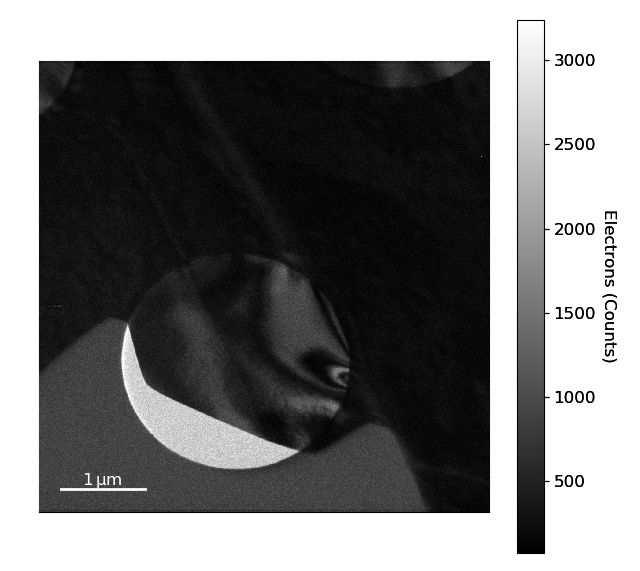
\includegraphics[width= 1 \linewidth]{img/tem_bf}
				\caption{Hellfeld}
		\end{subfigure}
	\begin{subfigure}[b]{0.45\textwidth}
				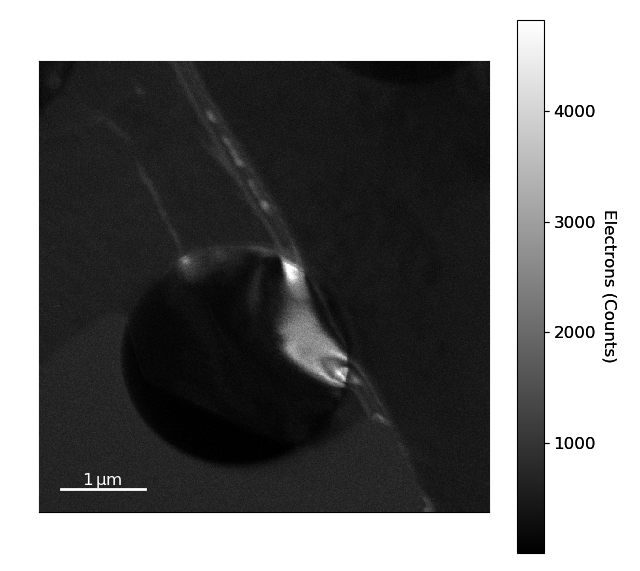
\includegraphics[width= 1 \linewidth]{img/tem_df}
				\caption{Dunkelfeld}
		\end{subfigure}
		\label{fig:tem_dfbf}
		\caption{
      Hell- und Dunkelfeld-Aufnahmen im TEM. Die runde Form ist ein Loch im membranartigen Probenhalter. Im Hellfeld ist der WSe$_2$-Kristall über dem Loch in dunkler Farbe erkennbar. Im Dunkelfeld ist in heller Farbe sichtbar, wo der Kristall besonders dick ist.
				}
	\end{figure}


 %TODO HRTEM: Aus Bild Netzebenenabstand bestimmen und aus FT von Bild.
 %TODO Gitterkonstante, Netzebenenabstand oder Atomabstand?

 \subsection{Bestimmung der Gitterkonstante}

 In \cref{fig:hrtem} ist die Aufnahme der Oberfläche des Kristalls dargestellt.
 Daraus wird durch Abzählen der Täler im Linienprofil die Gitterkonstante in den beiden sichtbaren Richtungen bestimmt und in \cref{tab:netz} dargestellt.
 Die Unsicherheit wurde mit einer Abweichung von einer Gitterkonstante über \SI{22}{} abgezählte Täler abgeschätzt.

	\begin{figure}[H]
		\centering
	\begin{subfigure}[b]{0.45\textwidth}
				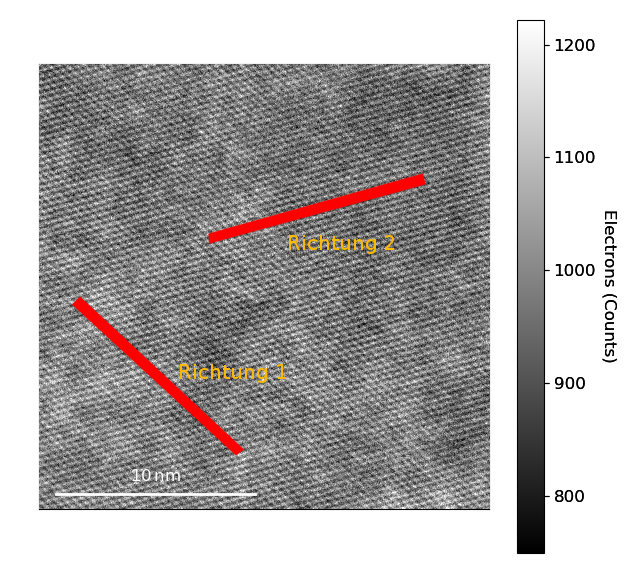
\includegraphics[width= 1 \linewidth]{img/hrtem_richt}
				\caption{}
		\end{subfigure}
	\begin{subfigure}[b]{0.45\textwidth}
				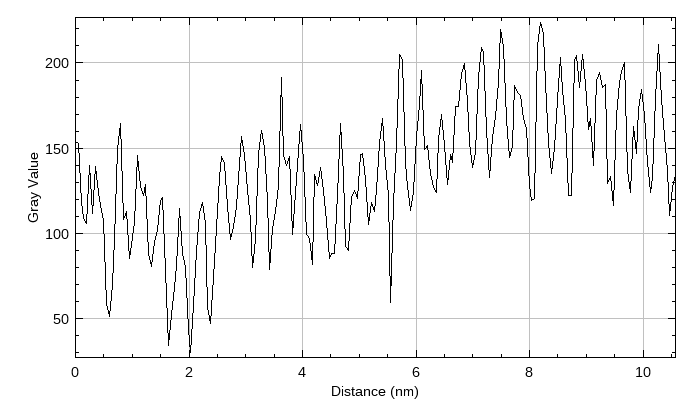
\includegraphics[width= 1 \linewidth]{img/tem_line-Plot_hrtem_zoom_crop}
				\caption{}
		\end{subfigure}
		\label{fig:hrtem}
		\caption{
      TEM-Aufnahme der Oberfläche des WSe$_2$-Kristalls und eines der Linienprofile.
				}
	\end{figure}

  Für \cref{fig:ft} wurde diese Aufnahme fouriertransformiert.
  Darin tauchen räumliche Frequenzen (die Gitterstruktur) als helle Punkte auf.
  Aus der Position dieser Punkte ergibt sich die räumliche Wellenlänge, die hier der Gitterkonstante entspricht.
  Die so ermittelten Gitterkonstanten sind in \cref{tab:netz} eingetragen.
  Für die Unsicherheit wurde die FWHM der röumlichen Peaks verwendet.

	\begin{figure}[H]
  \centering
			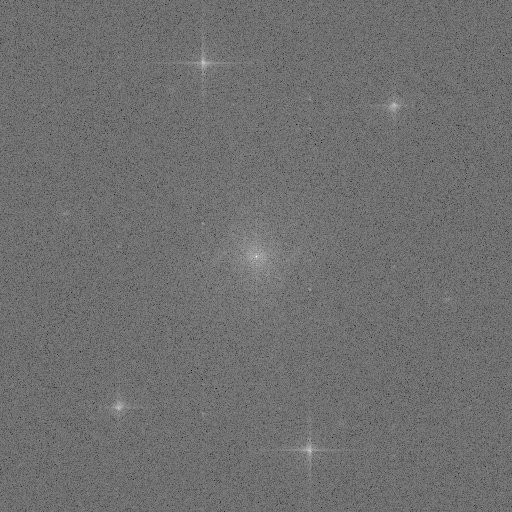
\includegraphics[width= 0.4 \linewidth]{img/tem_hrtem_crop_fft}
			\caption{
        Räumliche Fouriertransformation der TEM-Aufnahme in \cref{fig:hrtem}.
			}
			\label{fig:ft}
	\end{figure}

  Als letzte Methode wird das Bild in der Streuebene bei Beleuchtung einer hinreichend großen Fläche (einige Gitterkonstanten) aufgenommen und in \cref{fig:diff} abgebildet.
  Anhand der Abstände der Spots wird über den Kehrwert die Gitterkonstante des Realraumgitters bestimmt und in \cref{tab:netz} vermerkt.
  Es wird der Abstand über mehrere Spots gemessen und gemittelt.

	\begin{figure}[H]
  \centering
			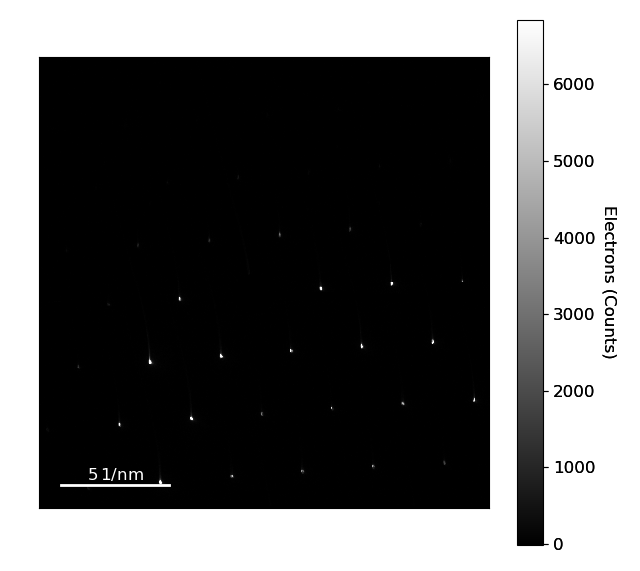
\includegraphics[width= 0.6 \linewidth]{img/tem_diff}
			\caption{
        TEM-Aufnahme der Streuebene.
			}
			\label{fig:diff}
	\end{figure}



	\begin{table}
		\centering
		\caption{Auf unterschiedliche Arten bestimmte Gitterkonstanten der Oberfläche der WSe$_2$-Probe. Die Richtungen können sind nur zu Unterscheidung innerhalb der selben Messmethode angegeben. Zwischen den Methoden sind die Richtungen nicht konstant.}
		\begin{tabular}{c| c | c}
			Methode & Richtung & Gitterkonstante \\ \hline
			% & & & \\
      Linienprofil &  1 & \SI{0.36 \pm 0.02}{nm}\\ %TODO hier ist was schiefgelaufen.
      Linienprofil &  2 & \SI{0.36 \pm 0.02}{nm}\\ %TODO neuer Wert: 0.29 überprüfen in Profil
      Fouriertransformation & 1 & \SI{0.29 \pm 0.01}{nm}\\
      & 2 & \SI{0.3 \pm 0.01}{nm}\\
      Streuebene & 1 & \SI{0,312 \pm 0.001}{nm} \\
      & 2 & \SI{0,317 \pm 0.001}{nm} \\
      & 3 & \SI{0,314 \pm 0.001}{nm} \\
      Mittelwert & & \\ %TODO mit Stderr
      Literatur & & \\ %TODO Litwert von Wikipedia
		\end{tabular}
		\label{tab:netz}
	\end{table}

  \subsection{EELS}

  Zuletzt wird das EEL-Spektrum der Probe aufgenommen.
  Es ist in zu sehen. %TODO
  Hier wurden die deutlich erkennbaren Peaks entsprechend ihres Ursprungs beschriftet.
 %TODO Im low-loss die Peaks zuordnen (im coreloss nur Silizium vom Trägermaterial sichtbar)
 %die Multimap-Dateien sind EFTEM-Aufnahmen. Da sollen wir nichts mit machen
